\documentclass[./main.tex]{subfiles} 
\begin{document}

\section{Non-parametric Spectrum Estimation}

\subsection{Discrete Fourier Transform Basics}

\subsubsection{}

\begin{figure}[h]
      \centering
      \begin{subfigure}[b]{0.49\textwidth}
         \resizebox{\textwidth}{!}{% This file was created by matlab2tikz v0.4.7 (commit 702a69c38ec8199e39ae3054d8e7897cd2bdae98) running on MATLAB 8.3.
% Copyright (c) 2008--2014, Nico Schlömer <nico.schloemer@gmail.com>
% All rights reserved.
% Minimal pgfplots version: 1.3
% 
% The latest updates can be retrieved from
%   http://www.mathworks.com/matlabcentral/fileexchange/22022-matlab2tikz
% where you can also make suggestions and rate matlab2tikz.
% 
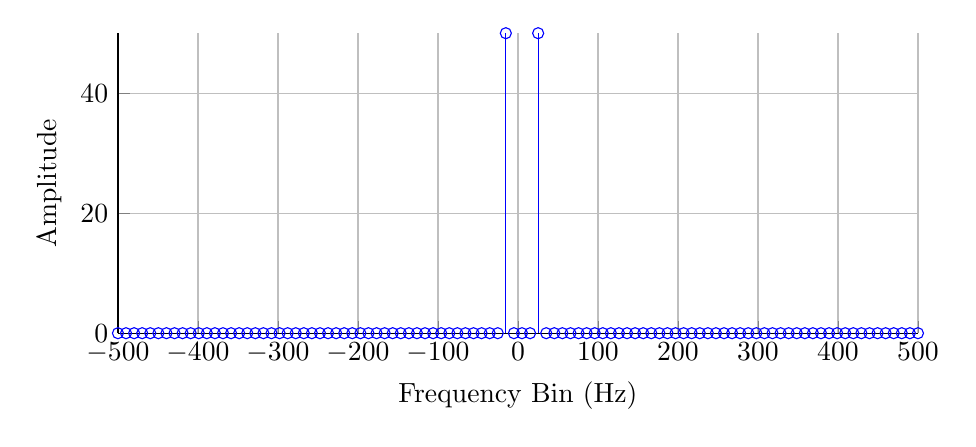
\begin{tikzpicture}

\begin{axis}[%
width=4in,
height=1.5in,
scale only axis,
xmin=-500,
xmax=500,
xlabel={Frequency Bin (Hz)},
xmajorgrids,
ymin=0,
ymax=50,
ylabel={Amplitude},
ymajorgrids,
axis x line*=bottom,
axis y line*=left
]
\addplot[ycomb,color=blue,solid,mark=o,mark options={solid}] plot table[row sep=crcr] {-500	1.11022302462516e-16\\
-489.89898989899	2.39470791920468e-16\\
-479.79797979798	3.97205464519564e-15\\
-469.69696969697	2.71287007248409e-15\\
-459.59595959596	3.61441376614477e-15\\
-449.494949494949	1.83323298352466e-15\\
-439.393939393939	4.89899281625692e-15\\
-429.292929292929	4.56294113517628e-15\\
-419.191919191919	1.65735141756668e-15\\
-409.090909090909	2.12112451432279e-15\\
-398.989898989899	2.3639378236e-15\\
-388.888888888889	1.57926540482738e-15\\
-378.787878787879	1.65735141756668e-15\\
-368.686868686869	2.75503365045881e-15\\
-358.585858585859	4.04239264171422e-15\\
-348.484848484849	4.3310038233772e-15\\
-338.383838383838	5.85657035135298e-15\\
-328.282828282828	5.75007177514217e-15\\
-318.181818181818	3.2580680567464e-15\\
-308.080808080808	4.60400367228801e-15\\
-297.979797979798	6.48938834789323e-15\\
-287.878787878788	6.23033209382719e-15\\
-277.777777777778	3.78476603133975e-15\\
-267.676767676768	2.53169801811368e-15\\
-257.575757575758	2.87485772981991e-15\\
-247.474747474747	4.37518032808405e-15\\
-237.373737373737	5.23570924248025e-15\\
-227.272727272727	3.33806235505672e-15\\
-217.171717171717	1.23580338698107e-15\\
-207.070707070707	1.06225410438752e-15\\
-196.969696969697	2.55985553021463e-15\\
-186.868686868687	9.62549166905435e-16\\
-176.767676767677	1.23580338698107e-15\\
-166.666666666667	1.27906841142066e-15\\
-156.565656565657	1.81949821949584e-15\\
-146.464646464646	2.21029480511369e-15\\
-136.363636363636	1.29088118847982e-15\\
-126.262626262626	1.43781691004488e-15\\
-116.161616161616	2.52085599615329e-15\\
-106.060606060606	3.21914436558581e-15\\
-95.959595959596	1.11274920914416e-15\\
-85.8585858585859	3.38326452522653e-15\\
-75.7575757575758	5.9388931498598e-16\\
-65.6565656565656	1.53145100772351e-15\\
-55.5555555555555	1.22183503710833e-15\\
-45.4545454545454	3.73404217251558e-15\\
-35.3535353535353	3.4333979636834e-15\\
-25.2525252525252	5.27306322948466e-15\\
-15.1515151515151	50\\
-5.05050505050502	2.47272494525015e-15\\
5.05050505050502	5.55111512312578e-16\\
15.1515151515151	2.47272494525015e-15\\
25.2525252525253	50\\
35.3535353535353	5.27306322948466e-15\\
45.4545454545455	3.4333979636834e-15\\
55.5555555555555	3.73404217251558e-15\\
65.6565656565657	1.22183503710833e-15\\
75.7575757575758	1.53145100772351e-15\\
85.8585858585859	5.9388931498598e-16\\
95.959595959596	3.38326452522653e-15\\
106.060606060606	1.11274920914416e-15\\
116.161616161616	3.21914436558581e-15\\
126.262626262626	2.52085599615329e-15\\
136.363636363636	1.43781691004488e-15\\
146.464646464646	1.29088118847982e-15\\
156.565656565657	2.21029480511369e-15\\
166.666666666667	1.81949821949584e-15\\
176.767676767677	1.27906841142066e-15\\
186.868686868687	1.23580338698107e-15\\
196.969696969697	9.62549166905435e-16\\
207.070707070707	2.55985553021463e-15\\
217.171717171717	1.06225410438752e-15\\
227.272727272727	1.23580338698107e-15\\
237.373737373737	3.33806235505672e-15\\
247.474747474747	5.23570924248025e-15\\
257.575757575758	4.37518032808405e-15\\
267.676767676768	2.87485772981991e-15\\
277.777777777778	2.53169801811368e-15\\
287.878787878788	3.78476603133975e-15\\
297.979797979798	6.23033209382719e-15\\
308.080808080808	6.48938834789323e-15\\
318.181818181818	4.60400367228801e-15\\
328.282828282828	3.2580680567464e-15\\
338.383838383838	5.75007177514217e-15\\
348.484848484849	5.85657035135298e-15\\
358.585858585859	4.3310038233772e-15\\
368.686868686869	4.04239264171422e-15\\
378.787878787879	2.75503365045881e-15\\
388.888888888889	1.65735141756668e-15\\
398.989898989899	1.57926540482738e-15\\
409.090909090909	2.3639378236e-15\\
419.191919191919	2.12112451432279e-15\\
429.292929292929	1.65735141756668e-15\\
439.393939393939	4.56294113517628e-15\\
449.49494949495	4.89899281625692e-15\\
459.59595959596	1.83323298352466e-15\\
469.69696969697	3.61441376614477e-15\\
479.79797979798	2.71287007248409e-15\\
489.89898989899	3.97205464519564e-15\\
500	2.39470791920468e-16\\
};
\addplot [color=black,solid,forget plot]
  table[row sep=crcr]{-500	0\\
500	0\\
};
\end{axis}
\end{tikzpicture}%}
  		\caption{\textit{1 Tree}}
  		\label{fig:1_1_b_100}
      \end{subfigure}
      ~ %add desired spacing between images, e. g. ~, \quad, \qquad, \hfill etc.
      \begin{subfigure}[b]{0.49\textwidth}
         \resizebox{\textwidth}{!}{% This file was created by matlab2tikz v0.4.7 (commit 702a69c38ec8199e39ae3054d8e7897cd2bdae98) running on MATLAB 8.3.
% Copyright (c) 2008--2014, Nico Schlömer <nico.schloemer@gmail.com>
% All rights reserved.
% Minimal pgfplots version: 1.3
% 
% The latest updates can be retrieved from
%   http://www.mathworks.com/matlabcentral/fileexchange/22022-matlab2tikz
% where you can also make suggestions and rate matlab2tikz.
% 
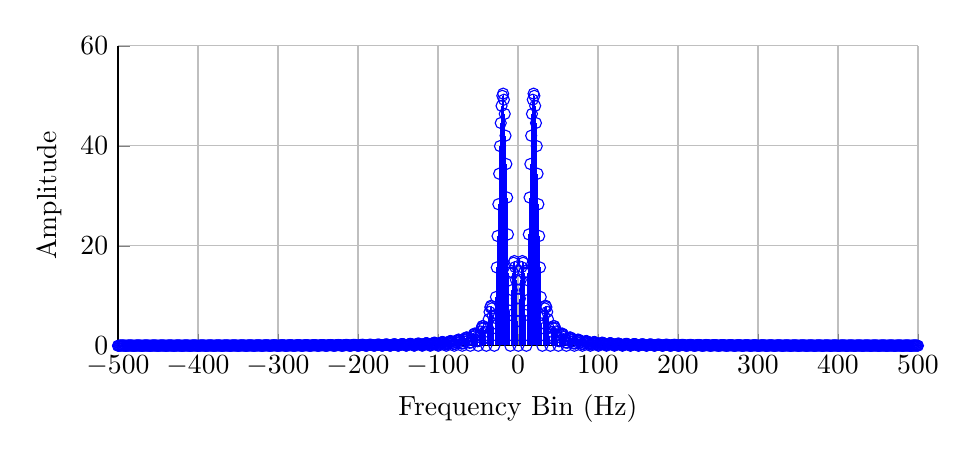
\begin{tikzpicture}

\begin{axis}[%
width=4in,
height=1.5in,
scale only axis,
xmin=-500,
xmax=500,
xlabel={Frequency Bin (Hz)},
xmajorgrids,
ymin=0,
ymax=60,
ylabel={Amplitude},
ymajorgrids,
axis x line*=bottom,
axis y line*=left
]
\addplot[ycomb,color=blue,solid,mark=o,mark options={solid}] plot table[row sep=crcr] {-500	1.11022302462516e-16\\
-498.998998998999	0.0194418940195181\\
-497.997997997998	0.0369817793064051\\
-496.996996996997	0.0509035743500947\\
-495.995995995996	0.059844891495999\\
-494.994994994995	0.06293025485105\\
-493.993993993994	0.0598567533646056\\
-492.992992992993	0.0509237557680847\\
-491.991991991992	0.0370037747504385\\
-490.990990990991	0.0194573137012285\\
-489.98998998999	2.39470791920468e-16\\
-488.988988988989	0.0194650296693576\\
-487.987987987988	0.0370331292049991\\
-486.986986986987	0.0509843641964171\\
-485.985985985986	0.0599517614891045\\
-484.984984984985	0.063055141569738\\
-483.983983983984	0.0599874414782314\\
-482.982982982983	0.0510450690384605\\
-481.981981981982	0.0370992905729064\\
-480.980980980981	0.0195114114344241\\
-479.97997997998	4.78298716822545e-15\\
-478.978978978979	0.0195269048346238\\
-477.977977977978	0.0371582333245807\\
-476.976976976977	0.0511667687483777\\
-475.975975975976	0.0601782147144249\\
-474.974974974975	0.0633059101896336\\
-473.973973973974	0.0602379975766611\\
-472.972972972973	0.0512684815057071\\
-471.971971971972	0.0372690886964231\\
-470.970970970971	0.019604618927338\\
-469.96996996997	2.62029866100517e-15\\
-468.968968968969	0.0196280137327647\\
-467.967967967968	0.0373580914073661\\
-466.966966966967	0.0514522464165978\\
-465.965965965966	0.0605260627764359\\
-464.964964964965	0.063684568008447\\
-463.963963963964	0.0606104284885591\\
-462.962962962963	0.0515957837445017\\
-461.961961961962	0.0375145309125169\\
-460.960960960961	0.0197376842362225\\
-459.95995995996	3.61441376614477e-15\\
-458.958958958959	0.0197691690504458\\
-457.957957957958	0.0376343111352421\\
-456.956956956957	0.0518430955087316\\
-455.955955955956	0.0609981085015501\\
-454.954954954955	0.0641941688016562\\
-453.953953953954	0.06110774051468\\
-452.952952952953	0.0520296202645944\\
-451.951951951952	0.0378376022550105\\
-450.950950950951	0.0199116846170306\\
-449.94994994995	1.83323298352466e-15\\
-448.948948948949	0.0199515159340171\\
-447.947947947948	0.0379891358357978\\
-446.946946946947	0.0523424938814769\\
-445.945945945946	0.0615981943502431\\
-444.944944944945	0.064838865632146\\
-443.943943943944	0.0617339914805952\\
-442.942942942943	0.0525735353576092\\
-441.941941941942	0.0382409454589661\\
-440.940940940941	0.0201280452511995\\
-439.93993993994	4.89899281625692e-15\\
-438.938938938939	0.0201765519514959\\
-437.937937937938	0.0384254836451673\\
-436.936936936937	0.0529545545017542\\
-435.935935935936	0.0623312697020978\\
-434.934934934935	0.0656239836896455\\
-433.933933933934	0.0624943620215602\\
-432.932932932933	0.0532320354642088\\
-431.931931931932	0.03872790754281\\
-430.930930930931	0.0203885644103379\\
-429.92992992993	4.46867522940645e-15\\
-428.928928928929	0.0204461536308439\\
-427.927927927928	0.0389469993160941\\
-426.926926926927	0.0536843986059851\\
-425.925925925926	0.0632034790630324\\
-424.924924924925	0.0665561153827653\\
-423.923923923924	0.0633952482792297\\
-422.922922922923	0.0540106699726147\\
-421.921921921922	0.0393025999441206\\
-420.920920920921	0.0206954458343536\\
-419.91991991992	2.49888694142632e-15\\
-418.918918918919	0.0207626103944635\\
-417.917917917918	0.0395581202757863\\
-416.916916916917	0.0545382487288748\\
-415.915915915916	0.0642222739399014\\
-414.914914914915	0.0676432406503704\\
-413.913913913914	0.0644443789093591\\
-412.912912912913	0.054916132981992\\
-411.911911911912	0.0399699740993928\\
-410.910910910911	0.0210513393433702\\
-409.90990990991	2.12112451432279e-15\\
-408.908908908909	0.0211286669654267\\
-407.907907907908	0.0402641590328201\\
-406.906906906907	0.0555235445661144\\
-405.905905905906	0.0653965519574538\\
-404.904904904905	0.0688948763478525\\
-403.903903903904	0.06565096016119\\
-402.902902902903	0.0559563893108758\\
-401.901901901902	0.0407359149114424\\
-400.900900900901	0.0214593910005468\\
-399.8998998999	2.3639378236e-15\\
-398.898898898899	0.0215475756290714\\
-397.897897897898	0.0410714046302718\\
-396.896896896897	0.0566490854754583\\
-395.895895895896	0.0667368278004401\\
-394.894894894895	0.0703222596454274\\
-393.893893893894	0.0670258538390895\\
-392.892892892893	0.0571408289430598\\
-391.891891891892	0.0416073552245013\\
-390.890890890891	0.021923304505982\\
-389.88988988989	1.57926540482738e-15\\
-388.888888888889	0.0220231601126423\\
-387.887887887888	0.0419872465791914\\
-386.886886886887	0.0579252044567413\\
-385.885885885886	0.0682554418084618\\
-384.884884884885	0.0719385717135415\\
-383.883883883884	0.068581794257842\\
-382.882882882883	0.0584804552342512\\
-381.881881881882	0.042592415267558\\
-380.880880880881	0.0224474159538264\\
-379.87987987988	2.49888694142632e-15\\
-378.878878878879	0.0225598933185164\\
-377.877877877878	0.0430203256261819\\
-376.876876876877	0.0593639797468292\\
-375.875875875876	0.0699668136093504\\
-374.874874874875	0.0737592096468967\\
-373.873873873874	0.0703336519349135\\
-372.872872872873	0.0599881136240348\\
-371.871871871872	0.0437005720833218\\
-370.870870870871	0.0230367846535034\\
-369.86986986987	3.15821892237082e-15\\
-368.868868868869	0.0231629917428244\\
-367.867867867868	0.0441807168707628\\
-366.866866866867	0.0609794918031427\\
-365.865865865866	0.0718877501490293\\
-364.864864864865	0.0758021167030984\\
-363.863863863864	0.0722987538328786\\
-362.862862862863	0.0616787694016932\\
-361.861861861862	0.0449428653033654\\
-360.860860860861	0.0236973034397094\\
-359.85985985986	4.04239264171422e-15\\
-358.858858858859	0.0238385301715683\\
-357.857857857858	0.0454801522305385\\
-356.856856856857	0.0627881355413564\\
-355.855855855856	0.0740378199969891\\
-354.854854854855	0.078088183650103\\
-353.853853853854	0.074497272616393\\
-352.852852852853	0.0635698453872083\\
-351.851851851852	0.0463321473534615\\
-350.850850850851	0.024435832825109\\
-349.84984984985	4.3310038233772e-15\\
-348.848848848849	0.0245935812245429\\
-347.847847847848	0.0469322911612361\\
-346.846846846847	0.0648090003888295\\
-345.845845845846	0.0764398090591453\\
-344.844844844845	0.0806417375264788\\
-343.843843843844	0.0769527008140191\\
-342.842842842843	0.0656816333804154\\
-341.841841841842	0.0478833884042908\\
-340.840840840841	0.0252603645540737\\
-339.83983983984	5.85657035135298e-15\\
-338.838838838839	0.0254363855869467\\
-337.837837837838	0.0485530510184745\\
-336.836836836837	0.0670643342207167\\
-335.835835835836	0.0791202770619634\\
-334.834834834835	0.0834911386893982\\
-333.833833833834	0.0796924302409917\\
-332.832832832833	0.0680377971336781\\
-331.831831831832	0.0496140492959003\\
-330.830830830831	0.02618022168935\\
-329.82982982983	6.12188219508283e-15\\
-328.828828828829	0.0263765604303437\\
-327.827827827828	0.0503610116969747\\
-326.826826826827	0.0695801118419189\\
-325.825825825826	0.0821102397261244\\
-324.824824824825	0.0866695130291727\\
-323.823823823824	0.0827484629095796\\
-322.822822822823	0.0706659897383252\\
-321.821821821822	0.0515445395004063\\
-320.820820820821	0.0272063044376788\\
-319.81981981982	3.7035444489294e-15\\
-318.818818818819	0.0274253557186964\\
-317.817817817818	0.0523779134757727\\
-316.816816816817	0.0723867347564918\\
-315.815815815816	0.0854460088996318\\
-314.814814814815	0.0902156541827402\\
-313.813813813814	0.0861582874375238\\
-312.812812812813	0.0735986151290724\\
-311.811811811812	0.0536987822826529\\
-310.810810810811	0.0283513936774566\\
-309.80980980981	4.60400367228801e-15\\
-308.808808808809	0.0285959710174039\\
-307.807807807808	0.054629272720534\\
-306.806806806807	0.0755198970761345\\
-305.805805805806	0.0891702327377732\\
-304.804804804805	0.0941751412094122\\
-303.803803803804	0.0899659653784069\\
-302.802802802803	0.076873772534929\\
-301.801801801802	0.0561049160477114\\
-300.800800800801	0.0296305278504795\\
-299.7997997998	6.48938834789323e-15\\
-298.798798798799	0.0299039493495871\\
-297.797797797798	0.0571451477907566\\
-296.796796796797	0.0790216633374069\\
-295.795795795796	0.0933331912467908\\
-294.794794794795	0.0986017315310888\\
-293.793793793794	0.0942234859565877\\
-292.792792792793	0.0805364350351485\\
-291.791791791792	0.0587961701008497\\
-290.790790790791	0.0310614738874465\\
-289.78978978979	6.23033209382719e-15\\
-288.788788788789	0.0313676699712559\\
-287.787787787788	0.0599610979519991\\
-286.786786786787	0.0829418188387702\\
-285.785785785786	0.0979944205086339\\
-284.784784784785	0.103559108468688\\
-283.783783783784	0.0989924668562066\\
-282.782782782783	0.0846399302056412\\
-281.781781781782	0.061811965664426\\
-280.780780780781	0.0326653196849674\\
-279.77977977978	4.06181318162096e-15\\
-278.778778778779	0.0330089692360947\\
-277.777777777778	0.0631193924296839\\
-276.776776776777	0.0873395734860962\\
-275.775775775776	0.103224763645542\\
-274.774774774775	0.109123089577517\\
-273.773773773774	0.104346305113919\\
-272.772772772773	0.0892478140428582\\
-271.771771771772	0.0651993104136033\\
-270.770770770771	0.034467225114364\\
-269.76976976977	2.53169801811368e-15\\
-268.768768768769	0.034853928828849\\
-267.767767767768	0.0666705466161806\\
-266.766766766767	0.0922857284168147\\
-265.765765765766	0.109108980959089\\
-264.764764764765	0.115384439360871\\
-263.763763763764	0.110372918927623\\
-262.762762762763	0.0944362616976003\\
-261.761761761762	0.0690145791024626\\
-260.760760760761	0.0364973817646178\\
-259.75975975976	2.87485772981991e-15\\
-258.758758758759	0.0369338848028337\\
-257.757757757758	0.0706752903111701\\
-256.756756756757	0.0978654543750321\\
-255.755755755756	0.115749099993077\\
-254.754754754755	0.122452482536414\\
-253.753753753754	0.117178272987568\\
-252.752752752753	0.100297144176976\\
-251.751751751752	0.0733258071846693\\
-250.750750750751	0.0387922503182768\\
-249.74974974975	4.37518032808405e-15\\
-248.748748748749	0.0392867309254015\\
-247.747747747748	0.0752071124303269\\
-246.746746746747	0.104181887232887\\
-245.745745745746	0.123268755020447\\
-244.744744744745	0.1304597889674\\
-243.743743743744	0.124890953827293\\
-242.742742742743	0.106942025349099\\
-241.741741741742	0.078215673441223\\
-240.740740740741	0.0413961712374859\\
-239.73973973974	5.23570924248025e-15\\
-238.738738738739	0.0419586186551296\\
-237.737737737738	0.0803555834995243\\
-236.736736736737	0.111360827303031\\
-235.735735735736	0.13181886459171\\
-234.734734734735	0.13956830957963\\
-233.733733733734	0.13366816853894\\
-232.732732732733	0.114507407962982\\
-231.731731731732	0.0837854188396181\\
-230.730730730731	0.0443634833238613\\
-229.72972972973	3.78128336773784e-15\\
-228.728728728729	0.0450061980468489\\
-227.727727727728	0.0862307402136792\\
-226.726726726727	0.119556947763515\\
-225.725725725726	0.141585140802067\\
-224.724724724725	0.149977501111052\\
-223.723723723724	0.143703696964843\\
-222.722722722723	0.123161696079446\\
-221.721721721722	0.0901600536511721\\
-220.720720720721	0.047761342034028\\
-219.71971971972	1.05407575513941e-15\\
-218.718718718719	0.0484996059408317\\
-217.717717717718	0.0929689392017306\\
-216.716716716717	0.128962093551103\\
-215.715715715716	0.152798139391148\\
-214.714714714715	0.161935213447785\\
-213.713713713714	0.155238561149541\\
-212.712712712713	0.133114548367439\\
-211.711711711712	0.0974953615877708\\
-210.710710710711	0.0516735152971698\\
-209.70970970971	1.06225410438752e-15\\
-208.708708708709	0.0525265010786672\\
-207.707707707708	0.100740772138861\\
-206.706706706707	0.139816517604441\\
-205.705705705706	0.165746885348756\\
-204.704704704705	0.175752470391796\\
-203.703703703704	0.168575530178025\\
-202.702702702703	0.144629611271433\\
-201.701701701702	0.105987448254442\\
-200.700700700701	0.0562055654989067\\
-199.6996996997	2.55985553021463e-15\\
-198.698698698699	0.0571975885517482\\
-197.697697697698	0.10976191800184\\
-196.696696696697	0.15242430923663\\
-195.695695695696	0.180797609783402\\
-194.694694694695	0.191823825387869\\
-193.693693693694	0.18409912603775\\
-192.692692692693	0.158042108045716\\
-191.691691691692	0.115885951252789\\
-190.690690690691	0.061492029797283\\
-189.68968968969	9.62549166905436e-16\\
-188.688688688689	0.0626542988106945\\
-187.687687687688	0.120308251903562\\
-186.686686686687	0.167174908710661\\
-185.685685685686	0.198419920812287\\
-184.684684684685	0.21065584048482\\
-183.683683683684	0.202303659756244\\
-182.682682682683	0.173783529473967\\
-181.681681681682	0.127512615504154\\
-180.680680680681	0.0677065340498478\\
-179.67967967968	1.05407575513941e-15\\
-178.678678678679	0.0690796418501246\\
-177.677677677678	0.132737239137021\\
-176.676676676677	0.184573626415329\\
-175.675675675676	0.21922399516826\\
-174.674674674675	0.232907632099598\\
-173.673673673674	0.223833220629396\\
-172.672672672673	0.192416917301862\\
-171.671671671672	0.141287887918848\\
-170.670670670671	0.0750763008356145\\
-169.66966966967	8.87998017683575e-16\\
-168.668668668669	0.0767138377378509\\
-167.667667667668	0.147518804532258\\
-166.666666666667	0.205285766918536\\
-165.665665665666	0.244014457913952\\
-164.664664664665	0.259449730112787\\
-163.663663663664	0.249539847560627\\
-162.662662662663	0.214688297630798\\
-161.661661661662	0.157769767108947\\
-160.660660660661	0.0839033883069058\\
-159.65965965966	1.81949821949584e-15\\
-158.658658658659	0.0858772986638753\\
-157.657657657658	0.165280821380953\\
-156.656656656657	0.230201796017116\\
-155.655655655656	0.273870138609561\\
-154.654654654655	0.291451405342286\\
-153.653653653654	0.280570037186121\\
-152.652652652653	0.241603349244508\\
-151.651651651652	0.1777118523233\\
-150.650650650651	0.0945965018279527\\
-149.64964964965	2.21029480511369e-15\\
-148.648648648649	0.0970052213357628\\
-147.647647647648	0.186877752879767\\
-146.646646646647	0.2605359259101\\
-145.645645645646	0.310265037743736\\
-144.644644644645	0.330513464950432\\
-143.643643643644	0.318496641035074\\
-142.642642642643	0.274544611279929\\
-141.641641641642	0.202152327308179\\
-140.640640640641	0.107719892494603\\
-139.63963963964	1.29088118847982e-15\\
-138.638638638639	0.110701058710059\\
-137.637637637638	0.213497059560528\\
-136.636636636637	0.297979384864097\\
-135.635635635636	0.355256945984764\\
-134.634634634635	0.378875934327781\\
-133.633633633634	0.365525767045172\\
-132.632632632633	0.315455906441565\\
-131.631631631632	0.232554410129236\\
-130.630630630631	0.124070781126041\\
-129.62962962963	2.22918029302773e-15\\
-128.628628628629	0.127821732659544\\
-127.627627627628	0.246829330096104\\
-126.626626626627	0.344946295200536\\
-125.625625625626	0.411791059537901\\
-124.624624624625	0.439753511088557\\
-123.623623623624	0.424832144419267\\
-122.622622622623	0.367142334903632\\
-121.621621621622	0.271035643110007\\
-120.620620620621	0.14480622007893\\
-119.61961961962	2.28259361945963e-15\\
-118.618618618619	0.14961830959357\\
-117.617617617618	0.289350227781258\\
-116.616616616617	0.40498274510063\\
-115.615615615616	0.484207119885751\\
-114.614614614615	0.517898151743238\\
-113.613613613614	0.501123873154706\\
-112.612612612613	0.433777571756146\\
-111.611611611612	0.320757276769237\\
-110.610610610611	0.171659463937119\\
-109.60960960961	3.21914436558581e-15\\
-108.608608608609	0.177978066489259\\
-107.607607607608	0.344807857989454\\
-106.606606606607	0.483477183055943\\
-105.605605605606	0.579124272940457\\
-104.604604604605	0.620585396139585\\
-103.603603603604	0.601637390695249\\
-102.602602602603	0.521802075536618\\
-101.601601601602	0.386617208992012\\
-100.600600600601	0.207327013236872\\
-99.5995995995996	1.11274920914416e-15\\
-98.5985985985986	0.215862129299832\\
-97.5975975975976	0.41910873253856\\
-96.5965965965966	0.58895904587653\\
-95.5955955955956	0.707067867130534\\
-94.5945945945946	0.759438279901896\\
-93.5935935935936	0.737988314215585\\
-92.5925925925926	0.641604091189562\\
-91.5915915915916	0.476554870290157\\
-90.5905905905906	0.256202081359457\\
-89.5895895895896	3.38326452522653e-15\\
-88.5885885885886	0.268145711168642\\
-87.5875875875876	0.522030270091075\\
-86.5865865865866	0.735626265643306\\
-85.5855855855856	0.885658071507492\\
-84.5845845845846	0.954028181446971\\
-83.5835835835836	0.929852519275526\\
-82.5825825825826	0.810888293655541\\
-81.5815815815816	0.60418645420462\\
-80.5805805805806	0.325867623628381\\
-79.5795795795796	8.41858542412078e-16\\
-78.5785785785786	0.343356839981742\\
-77.5775775775776	0.670794895099069\\
-76.5765765765766	0.948666728577203\\
-75.5755755755756	1.14638384106911\\
-74.5745745745746	1.23959542271224\\
-73.5735735735736	1.21293389139457\\
-72.5725725725726	1.0620385884783\\
-71.5715715715716	0.794622624892997\\
-70.5705705705706	0.430426536763381\\
-69.5695695695696	6.73333721719995e-16\\
-68.5685685685686	0.457638809749534\\
-67.5675675675676	0.89830711615407\\
-66.5665665665666	1.27666507796637\\
-65.5655655655656	1.55058562440701\\
-64.5645645645646	1.68549093719456\\
-63.5635635635635	1.65823950972919\\
-62.5625625625626	1.46016491764459\\
-61.5615615615616	1.09892272798445\\
-60.5605605605606	0.598892374250434\\
-59.5595595595595	1.22183503710833e-15\\
-58.5585585585586	0.645033047975316\\
-57.5575575575576	1.2748647377363\\
-56.5565565565565	1.82483675514703\\
-55.5555555555555	2.23299184343251\\
-54.5545545545546	2.44629345807426\\
-53.5535535535536	2.42648373700879\\
-52.5525525525525	2.15500981035735\\
-51.5515515515515	1.63649319656741\\
-50.5505505505506	0.900311457210902\\
-49.5495495495496	3.73404217251558e-15\\
-48.5485485485485	0.98964464187824\\
-47.5475475475475	1.9776836689819\\
-46.5465465465466	2.86409962568726\\
-45.5455455455456	3.54833744200134\\
-44.5445445445445	3.93869369199097\\
-43.5435435435435	3.96180645167478\\
-42.5425425425425	3.57143579595918\\
-41.5415415415416	2.75572715857089\\
-40.5405405405405	1.5422199572776\\
-39.5395395395395	3.4333979636834e-15\\
-38.5385385385385	1.7614114286196\\
-37.5375375375376	3.59659912925176\\
-36.5365365365365	5.33212563301839\\
-35.5355355355355	6.77735675558703\\
-34.5345345345345	7.73760357148222\\
-33.5335335335336	8.0287181683675\\
-32.5325325325325	7.49211148917462\\
-31.5315315315315	6.00906491943388\\
-30.5305305305305	3.5131942268046\\
-29.5295295295296	5.73054535427406e-15\\
-28.5285285285285	4.46739899361767\\
-27.5275275275275	9.75701292484531\\
-26.5265265265265	15.6715691087841\\
-25.5255255255256	21.9569573935337\\
-24.5245245245245	28.3151874669151\\
-23.5235235235235	34.4211617599754\\
-22.5225225225225	39.9422541724149\\
-21.5215215215215	44.5594343235225\\
-20.5205205205205	47.9885107556079\\
-19.5195195195195	50\\
-18.5185185185185	50.4361700021657\\
-17.5175175175175	49.2239564202793\\
-16.5165165165165	46.3827008351155\\
-15.5155155155155	42.0259951612575\\
-14.5145145145145	36.3573139245553\\
-13.5135135135135	29.6595477106004\\
-12.5125125125125	22.2789859001941\\
-11.5115115115115	14.6047027680495\\
-10.5105105105105	7.04464760063621\\
-9.50950950950948	2.47272494525015e-15\\
-8.5085085085085	6.16049477207635\\
-7.50750750750751	11.1244618438891\\
-6.50650650650653	14.6564463185492\\
-5.50550550550548	16.6136289327952\\
-4.5045045045045	16.9555767629317\\
-3.50350350350351	15.7472987579399\\
-2.50250250250252	13.1553329335848\\
-1.50150150150148	9.43707282085205\\
-0.500500500500493	4.92401067288395\\
0.500500500500493	5.55111512312578e-16\\
1.50150150150148	4.92401067288395\\
2.50250250250252	9.43707282085205\\
3.50350350350351	13.1553329335848\\
4.5045045045045	15.7472987579399\\
5.50550550550548	16.9555767629317\\
6.50650650650653	16.6136289327952\\
7.50750750750751	14.6564463185492\\
8.5085085085085	11.1244618438891\\
9.50950950950948	6.16049477207635\\
10.5105105105105	2.47272494525015e-15\\
11.5115115115115	7.04464760063621\\
12.5125125125126	14.6047027680495\\
13.5135135135135	22.2789859001941\\
14.5145145145145	29.6595477106004\\
15.5155155155155	36.3573139245553\\
16.5165165165165	42.0259951612575\\
17.5175175175175	46.3827008351155\\
18.5185185185185	49.2239564202793\\
19.5195195195195	50.4361700021657\\
20.5205205205206	50\\
21.5215215215215	47.9885107556079\\
22.5225225225225	44.5594343235225\\
23.5235235235235	39.9422541724149\\
24.5245245245245	34.4211617599754\\
25.5255255255255	28.3151874669151\\
26.5265265265265	21.9569573935337\\
27.5275275275276	15.6715691087841\\
28.5285285285286	9.75701292484531\\
29.5295295295296	4.46739899361767\\
30.5305305305305	5.73054535427406e-15\\
31.5315315315315	3.5131942268046\\
32.5325325325325	6.00906491943388\\
33.5335335335335	7.49211148917462\\
34.5345345345345	8.0287181683675\\
35.5355355355356	7.73760357148222\\
36.5365365365366	6.77735675558703\\
37.5375375375376	5.33212563301839\\
38.5385385385385	3.59659912925176\\
39.5395395395395	1.7614114286196\\
40.5405405405405	3.4333979636834e-15\\
41.5415415415415	1.5422199572776\\
42.5425425425425	2.75572715857089\\
43.5435435435436	3.57143579595918\\
44.5445445445446	3.96180645167478\\
45.5455455455456	3.93869369199097\\
46.5465465465466	3.54833744200134\\
47.5475475475475	2.86409962568726\\
48.5485485485485	1.9776836689819\\
49.5495495495495	0.98964464187824\\
50.5505505505505	3.73404217251558e-15\\
51.5515515515516	0.900311457210902\\
52.5525525525526	1.63649319656741\\
53.5535535535536	2.15500981035735\\
54.5545545545546	2.42648373700879\\
55.5555555555555	2.44629345807426\\
56.5565565565565	2.23299184343251\\
57.5575575575575	1.82483675514703\\
58.5585585585585	1.2748647377363\\
59.5595595595596	0.645033047975316\\
60.5605605605606	1.22183503710833e-15\\
61.5615615615616	0.598892374250434\\
62.5625625625626	1.09892272798445\\
63.5635635635635	1.46016491764459\\
64.5645645645645	1.65823950972919\\
65.5655655655655	1.68549093719456\\
66.5665665665666	1.55058562440701\\
67.5675675675676	1.27666507796637\\
68.5685685685686	0.89830711615407\\
69.5695695695696	0.457638809749534\\
70.5705705705706	6.73333721719995e-16\\
71.5715715715716	0.430426536763381\\
72.5725725725725	0.794622624892997\\
73.5735735735735	1.0620385884783\\
74.5745745745746	1.21293389139457\\
75.5755755755756	1.23959542271224\\
76.5765765765766	1.14638384106911\\
77.5775775775776	0.948666728577203\\
78.5785785785786	0.670794895099069\\
79.5795795795796	0.343356839981742\\
80.5805805805805	8.41858542412078e-16\\
81.5815815815815	0.325867623628381\\
82.5825825825826	0.60418645420462\\
83.5835835835836	0.810888293655541\\
84.5845845845846	0.929852519275526\\
85.5855855855856	0.954028181446971\\
86.5865865865866	0.885658071507492\\
87.5875875875876	0.735626265643306\\
88.5885885885886	0.522030270091075\\
89.5895895895895	0.268145711168642\\
90.5905905905906	3.38326452522653e-15\\
91.5915915915916	0.256202081359457\\
92.5925925925926	0.476554870290157\\
93.5935935935936	0.641604091189562\\
94.5945945945946	0.737988314215585\\
95.5955955955956	0.759438279901896\\
96.5965965965966	0.707067867130534\\
97.5975975975975	0.58895904587653\\
98.5985985985986	0.41910873253856\\
99.5995995995996	0.215862129299832\\
100.600600600601	1.11274920914416e-15\\
101.601601601602	0.207327013236872\\
102.602602602603	0.386617208992012\\
103.603603603604	0.521802075536618\\
104.604604604605	0.601637390695249\\
105.605605605606	0.620585396139585\\
106.606606606607	0.579124272940457\\
107.607607607608	0.483477183055943\\
108.608608608609	0.344807857989454\\
109.60960960961	0.177978066489259\\
110.610610610611	3.21914436558581e-15\\
111.611611611612	0.171659463937119\\
112.612612612613	0.320757276769237\\
113.613613613614	0.433777571756146\\
114.614614614615	0.501123873154706\\
115.615615615616	0.517898151743238\\
116.616616616617	0.484207119885751\\
117.617617617618	0.40498274510063\\
118.618618618619	0.289350227781258\\
119.61961961962	0.14961830959357\\
120.620620620621	2.28259361945963e-15\\
121.621621621622	0.14480622007893\\
122.622622622623	0.271035643110007\\
123.623623623624	0.367142334903632\\
124.624624624625	0.424832144419267\\
125.625625625626	0.439753511088557\\
126.626626626627	0.411791059537901\\
127.627627627628	0.344946295200536\\
128.628628628629	0.246829330096104\\
129.62962962963	0.127821732659544\\
130.630630630631	2.22918029302773e-15\\
131.631631631632	0.124070781126041\\
132.632632632633	0.232554410129236\\
133.633633633634	0.315455906441565\\
134.634634634635	0.365525767045172\\
135.635635635636	0.378875934327781\\
136.636636636637	0.355256945984764\\
137.637637637638	0.297979384864097\\
138.638638638639	0.213497059560528\\
139.63963963964	0.110701058710059\\
140.640640640641	1.29088118847982e-15\\
141.641641641642	0.107719892494603\\
142.642642642643	0.202152327308179\\
143.643643643644	0.274544611279929\\
144.644644644645	0.318496641035074\\
145.645645645646	0.330513464950432\\
146.646646646647	0.310265037743736\\
147.647647647648	0.2605359259101\\
148.648648648649	0.186877752879767\\
149.64964964965	0.0970052213357628\\
150.650650650651	2.21029480511369e-15\\
151.651651651652	0.0945965018279527\\
152.652652652653	0.1777118523233\\
153.653653653654	0.241603349244508\\
154.654654654655	0.280570037186121\\
155.655655655656	0.291451405342286\\
156.656656656657	0.273870138609561\\
157.657657657658	0.230201796017116\\
158.658658658659	0.165280821380953\\
159.65965965966	0.0858772986638753\\
160.660660660661	1.81949821949584e-15\\
161.661661661662	0.0839033883069058\\
162.662662662663	0.157769767108947\\
163.663663663664	0.214688297630798\\
164.664664664665	0.249539847560627\\
165.665665665666	0.259449730112787\\
166.666666666667	0.244014457913952\\
167.667667667668	0.205285766918536\\
168.668668668669	0.147518804532258\\
169.66966966967	0.0767138377378509\\
170.670670670671	8.87998017683575e-16\\
171.671671671672	0.0750763008356145\\
172.672672672673	0.141287887918848\\
173.673673673674	0.192416917301862\\
174.674674674675	0.223833220629396\\
175.675675675676	0.232907632099598\\
176.676676676677	0.21922399516826\\
177.677677677678	0.184573626415329\\
178.678678678679	0.132737239137021\\
179.67967967968	0.0690796418501246\\
180.680680680681	1.05407575513941e-15\\
181.681681681682	0.0677065340498478\\
182.682682682683	0.127512615504154\\
183.683683683684	0.173783529473967\\
184.684684684685	0.202303659756244\\
185.685685685686	0.21065584048482\\
186.686686686687	0.198419920812287\\
187.687687687688	0.167174908710661\\
188.688688688689	0.120308251903562\\
189.68968968969	0.0626542988106945\\
190.690690690691	9.62549166905436e-16\\
191.691691691692	0.061492029797283\\
192.692692692693	0.115885951252789\\
193.693693693694	0.158042108045716\\
194.694694694695	0.18409912603775\\
195.695695695696	0.191823825387869\\
196.696696696697	0.180797609783402\\
197.697697697698	0.15242430923663\\
198.698698698699	0.10976191800184\\
199.6996996997	0.0571975885517482\\
200.700700700701	2.55985553021463e-15\\
201.701701701702	0.0562055654989067\\
202.702702702703	0.105987448254442\\
203.703703703704	0.144629611271433\\
204.704704704705	0.168575530178025\\
205.705705705706	0.175752470391796\\
206.706706706707	0.165746885348756\\
207.707707707708	0.139816517604441\\
208.708708708709	0.100740772138861\\
209.70970970971	0.0525265010786672\\
210.710710710711	1.06225410438752e-15\\
211.711711711712	0.0516735152971698\\
212.712712712713	0.0974953615877708\\
213.713713713714	0.133114548367439\\
214.714714714715	0.155238561149541\\
215.715715715716	0.161935213447785\\
216.716716716717	0.152798139391148\\
217.717717717718	0.128962093551103\\
218.718718718719	0.0929689392017306\\
219.71971971972	0.0484996059408317\\
220.720720720721	1.05407575513941e-15\\
221.721721721722	0.047761342034028\\
222.722722722723	0.0901600536511721\\
223.723723723724	0.123161696079446\\
224.724724724725	0.143703696964843\\
225.725725725726	0.149977501111052\\
226.726726726727	0.141585140802067\\
227.727727727728	0.119556947763515\\
228.728728728729	0.0862307402136792\\
229.72972972973	0.0450061980468489\\
230.730730730731	3.78128336773784e-15\\
231.731731731732	0.0443634833238613\\
232.732732732733	0.0837854188396181\\
233.733733733734	0.114507407962982\\
234.734734734735	0.13366816853894\\
235.735735735736	0.13956830957963\\
236.736736736737	0.13181886459171\\
237.737737737738	0.111360827303031\\
238.738738738739	0.0803555834995243\\
239.73973973974	0.0419586186551296\\
240.740740740741	5.23570924248025e-15\\
241.741741741742	0.0413961712374859\\
242.742742742743	0.078215673441223\\
243.743743743744	0.106942025349099\\
244.744744744745	0.124890953827293\\
245.745745745746	0.1304597889674\\
246.746746746747	0.123268755020447\\
247.747747747748	0.104181887232887\\
248.748748748749	0.0752071124303269\\
249.74974974975	0.0392867309254015\\
250.750750750751	4.37518032808405e-15\\
251.751751751752	0.0387922503182768\\
252.752752752753	0.0733258071846693\\
253.753753753754	0.100297144176976\\
254.754754754755	0.117178272987568\\
255.755755755756	0.122452482536414\\
256.756756756757	0.115749099993077\\
257.757757757758	0.0978654543750321\\
258.758758758759	0.0706752903111701\\
259.75975975976	0.0369338848028337\\
260.760760760761	2.87485772981991e-15\\
261.761761761762	0.0364973817646178\\
262.762762762763	0.0690145791024626\\
263.763763763764	0.0944362616976003\\
264.764764764765	0.110372918927623\\
265.765765765766	0.115384439360871\\
266.766766766767	0.109108980959089\\
267.767767767768	0.0922857284168147\\
268.768768768769	0.0666705466161806\\
269.76976976977	0.034853928828849\\
270.770770770771	2.53169801811368e-15\\
271.771771771772	0.034467225114364\\
272.772772772773	0.0651993104136033\\
273.773773773774	0.0892478140428582\\
274.774774774775	0.104346305113919\\
275.775775775776	0.109123089577517\\
276.776776776777	0.103224763645542\\
277.777777777778	0.0873395734860962\\
278.778778778779	0.0631193924296839\\
279.77977977978	0.0330089692360947\\
280.780780780781	4.06181318162096e-15\\
281.781781781782	0.0326653196849674\\
282.782782782783	0.061811965664426\\
283.783783783784	0.0846399302056412\\
284.784784784785	0.0989924668562066\\
285.785785785786	0.103559108468688\\
286.786786786787	0.0979944205086339\\
287.787787787788	0.0829418188387702\\
288.788788788789	0.0599610979519991\\
289.78978978979	0.0313676699712559\\
290.790790790791	6.23033209382719e-15\\
291.791791791792	0.0310614738874465\\
292.792792792793	0.0587961701008497\\
293.793793793794	0.0805364350351485\\
294.794794794795	0.0942234859565877\\
295.795795795796	0.0986017315310888\\
296.796796796797	0.0933331912467908\\
297.797797797798	0.0790216633374069\\
298.798798798799	0.0571451477907566\\
299.7997997998	0.0299039493495871\\
300.800800800801	6.48938834789323e-15\\
301.801801801802	0.0296305278504795\\
302.802802802803	0.0561049160477114\\
303.803803803804	0.076873772534929\\
304.804804804805	0.0899659653784069\\
305.805805805806	0.0941751412094122\\
306.806806806807	0.0891702327377732\\
307.807807807808	0.0755198970761345\\
308.808808808809	0.054629272720534\\
309.80980980981	0.0285959710174039\\
310.810810810811	4.60400367228801e-15\\
311.811811811812	0.0283513936774566\\
312.812812812813	0.0536987822826529\\
313.813813813814	0.0735986151290724\\
314.814814814815	0.0861582874375238\\
315.815815815816	0.0902156541827402\\
316.816816816817	0.0854460088996318\\
317.817817817818	0.0723867347564918\\
318.818818818819	0.0523779134757727\\
319.81981981982	0.0274253557186964\\
320.820820820821	3.7035444489294e-15\\
321.821821821822	0.0272063044376788\\
322.822822822823	0.0515445395004063\\
323.823823823824	0.0706659897383252\\
324.824824824825	0.0827484629095796\\
325.825825825826	0.0866695130291727\\
326.826826826827	0.0821102397261244\\
327.827827827828	0.0695801118419189\\
328.828828828829	0.0503610116969747\\
329.82982982983	0.0263765604303437\\
330.830830830831	6.12188219508283e-15\\
331.831831831832	0.02618022168935\\
332.832832832833	0.0496140492959003\\
333.833833833834	0.0680377971336781\\
334.834834834835	0.0796924302409917\\
335.835835835836	0.0834911386893982\\
336.836836836837	0.0791202770619634\\
337.837837837838	0.0670643342207167\\
338.838838838839	0.0485530510184745\\
339.83983983984	0.0254363855869467\\
340.840840840841	5.85657035135298e-15\\
341.841841841842	0.0252603645540737\\
342.842842842843	0.0478833884042908\\
343.843843843844	0.0656816333804154\\
344.844844844845	0.0769527008140191\\
345.845845845846	0.0806417375264788\\
346.846846846847	0.0764398090591453\\
347.847847847848	0.0648090003888295\\
348.848848848849	0.0469322911612361\\
349.84984984985	0.0245935812245429\\
350.850850850851	4.3310038233772e-15\\
351.851851851852	0.024435832825109\\
352.852852852853	0.0463321473534615\\
353.853853853854	0.0635698453872083\\
354.854854854855	0.074497272616393\\
355.855855855856	0.078088183650103\\
356.856856856857	0.0740378199969891\\
357.857857857858	0.0627881355413564\\
358.858858858859	0.0454801522305385\\
359.85985985986	0.0238385301715683\\
360.860860860861	4.04239264171422e-15\\
361.861861861862	0.0236973034397094\\
362.862862862863	0.0449428653033654\\
363.863863863864	0.0616787694016932\\
364.864864864865	0.0722987538328786\\
365.865865865866	0.0758021167030984\\
366.866866866867	0.0718877501490293\\
367.867867867868	0.0609794918031427\\
368.868868868869	0.0441807168707628\\
369.86986986987	0.0231629917428244\\
370.870870870871	3.15821892237082e-15\\
371.871871871872	0.0230367846535034\\
372.872872872873	0.0437005720833218\\
373.873873873874	0.0599881136240348\\
374.874874874875	0.0703336519349135\\
375.875875875876	0.0737592096468967\\
376.876876876877	0.0699668136093504\\
377.877877877878	0.0593639797468292\\
378.878878878879	0.0430203256261819\\
379.87987987988	0.0225598933185164\\
380.880880880881	2.49888694142632e-15\\
381.881881881882	0.0224474159538264\\
382.882882882883	0.042592415267558\\
383.883883883884	0.0584804552342512\\
384.884884884885	0.068581794257842\\
385.885885885886	0.0719385717135415\\
386.886886886887	0.0682554418084618\\
387.887887887888	0.0579252044567413\\
388.888888888889	0.0419872465791914\\
389.88988988989	0.0220231601126423\\
390.890890890891	1.57926540482738e-15\\
391.891891891892	0.021923304505982\\
392.892892892893	0.0416073552245013\\
393.893893893894	0.0571408289430598\\
394.894894894895	0.0670258538390895\\
395.895895895896	0.0703222596454274\\
396.896896896897	0.0667368278004401\\
397.897897897898	0.0566490854754583\\
398.898898898899	0.0410714046302718\\
399.8998998999	0.0215475756290714\\
400.900900900901	2.3639378236e-15\\
401.901901901902	0.0214593910005468\\
402.902902902903	0.0407359149114424\\
403.903903903904	0.0559563893108758\\
404.904904904905	0.06565096016119\\
405.905905905906	0.0688948763478525\\
406.906906906907	0.0653965519574538\\
407.907907907908	0.0555235445661144\\
408.908908908909	0.0402641590328201\\
409.90990990991	0.0211286669654267\\
410.910910910911	2.12112451432279e-15\\
411.911911911912	0.0210513393433702\\
412.912912912913	0.0399699740993928\\
413.913913913914	0.054916132981992\\
414.914914914915	0.0644443789093591\\
415.915915915916	0.0676432406503704\\
416.916916916917	0.0642222739399014\\
417.917917917918	0.0545382487288748\\
418.918918918919	0.0395581202757863\\
419.91991991992	0.0207626103944635\\
420.920920920921	2.49888694142632e-15\\
421.921921921922	0.0206954458343536\\
422.922922922923	0.0393025999441206\\
423.923923923924	0.0540106699726147\\
424.924924924925	0.0633952482792297\\
425.925925925926	0.0665561153827653\\
426.926926926927	0.0632034790630324\\
427.927927927928	0.0536843986059851\\
428.928928928929	0.0389469993160941\\
429.92992992993	0.0204461536308439\\
430.930930930931	4.46867522940645e-15\\
431.931931931932	0.0203885644103379\\
432.932932932933	0.03872790754281\\
433.933933933934	0.0532320354642088\\
434.934934934935	0.0624943620215602\\
435.935935935936	0.0656239836896455\\
436.936936936937	0.0623312697020978\\
437.937937937938	0.0529545545017542\\
438.938938938939	0.0384254836451673\\
439.93993993994	0.0201765519514959\\
440.940940940941	4.89899281625692e-15\\
441.941941941942	0.0201280452511995\\
442.942942942943	0.0382409454589661\\
443.943943943944	0.0525735353576092\\
444.944944944945	0.0617339914805952\\
445.945945945946	0.064838865632146\\
446.946946946947	0.0615981943502431\\
447.947947947948	0.0523424938814769\\
448.948948948949	0.0379891358357978\\
449.94994994995	0.0199515159340171\\
450.950950950951	1.83323298352466e-15\\
451.951951951952	0.0199116846170306\\
452.952952952953	0.0378376022550105\\
453.953953953954	0.0520296202645944\\
454.954954954955	0.06110774051468\\
455.955955955956	0.0641941688016562\\
456.956956956957	0.0609981085015501\\
457.957957957958	0.0518430955087316\\
458.958958958959	0.0376343111352421\\
459.95995995996	0.0197691690504458\\
460.960960960961	3.61441376614477e-15\\
461.961961961962	0.0197376842362225\\
462.962962962963	0.0375145309125169\\
463.963963963964	0.0515957837445017\\
464.964964964965	0.0606104284885591\\
465.965965965966	0.063684568008447\\
466.966966966967	0.0605260627764359\\
467.967967967968	0.0514522464165978\\
468.968968968969	0.0373580914073661\\
469.96996996997	0.0196280137327647\\
470.970970970971	2.62029866100517e-15\\
471.971971971972	0.019604618927338\\
472.972972972973	0.0372690886964231\\
473.973973973974	0.0512684815057071\\
474.974974974975	0.0602379975766611\\
475.975975975976	0.0633059101896336\\
476.976976976977	0.0601782147144249\\
477.977977977978	0.0511667687483777\\
478.978978978979	0.0371582333245807\\
479.97997997998	0.0195269048346238\\
480.980980980981	4.78298716822545e-15\\
481.981981981982	0.0195114114344241\\
482.982982982983	0.0370992905729064\\
483.983983983984	0.0510450690384605\\
484.984984984985	0.0599874414782314\\
485.985985985986	0.063055141569738\\
486.986986986987	0.0599517614891045\\
487.987987987988	0.0509843641964171\\
488.988988988989	0.0370331292049991\\
489.98998998999	0.0194650296693576\\
490.990990990991	2.39470791920468e-16\\
491.991991991992	0.0194573137012285\\
492.992992992993	0.0370037747504385\\
493.993993993994	0.0509237557680847\\
494.994994994995	0.0598567533646056\\
495.995995995996	0.06293025485105\\
496.996996996997	0.059844891495999\\
497.997997997998	0.0509035743500947\\
498.998998998999	0.0369817793064051\\
500	0.0194418940195181\\
};
\addplot [color=black,solid,forget plot]
  table[row sep=crcr]{-500	0\\
500	0\\
};
\end{axis}
\end{tikzpicture}%}
 			\caption{\textit{2 Trees}}
  		\label{fig:1_1_b_1000}
      \end{subfigure}
	\label{fig:1_1_b}
	\caption{\textit{DFTs of 20Hz Sine Wave, with $ F_s = 1000 $Hz}}
  \end{figure}

\subsubsection{Incoherent Sampling}

\begin{figure}[h]
	\centering 
	\resizebox{0.7\textwidth}{!}{% This file was created by matlab2tikz v0.4.7 (commit 702a69c38ec8199e39ae3054d8e7897cd2bdae98) running on MATLAB 8.3.
% Copyright (c) 2008--2014, Nico Schlömer <nico.schloemer@gmail.com>
% All rights reserved.
% Minimal pgfplots version: 1.3
% 
% The latest updates can be retrieved from
%   http://www.mathworks.com/matlabcentral/fileexchange/22022-matlab2tikz
% where you can also make suggestions and rate matlab2tikz.
% 
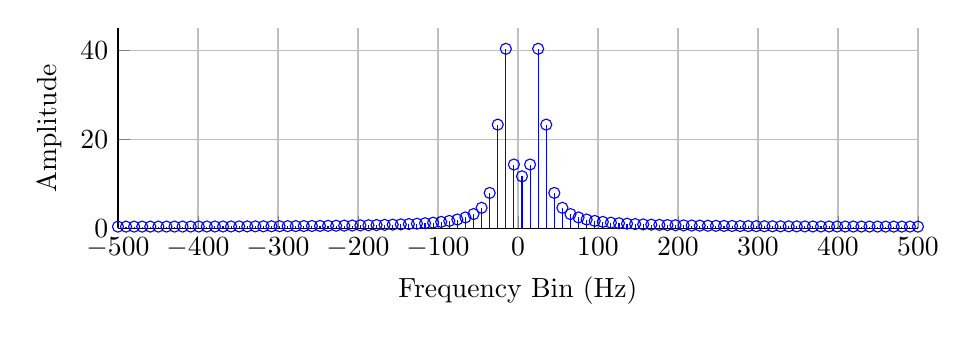
\begin{tikzpicture}

\begin{axis}[%
width=4in,
height=1in,
scale only axis,
xmin=-500,
xmax=500,
xlabel={Frequency Bin (Hz)},
xmajorgrids,
ymin=0,
ymax=45,
ylabel={Amplitude},
ymajorgrids,
axis x line*=bottom,
axis y line*=left
]
\addplot[ycomb,color=blue,solid,mark=o,mark options={solid}] plot table[row sep=crcr] {-500	0.362220488082982\\
-489.89898989899	0.362407411759151\\
-479.79797979798	0.362969178838951\\
-469.69696969697	0.363908790787336\\
-459.59595959596	0.36523129475414\\
-449.494949494949	0.366943851833486\\
-439.393939393939	0.369055835072228\\
-429.292929292929	0.371578959795506\\
-419.191919191919	0.374527449735377\\
-409.090909090909	0.377918243519789\\
-398.989898989899	0.381771247358408\\
-388.888888888889	0.386109641315216\\
-378.787878787879	0.390960248473884\\
-368.686868686869	0.396353978693896\\
-358.585858585859	0.402326361674905\\
-348.484848484849	0.408918187896029\\
-338.383838383838	0.416176280950324\\
-328.282828282828	0.424154431226743\\
-318.181818181818	0.43291452932051\\
-308.080808080808	0.442527948699865\\
-297.979797979798	0.453077242041048\\
-287.878787878788	0.464658235716285\\
-277.777777777778	0.477382634278217\\
-267.676767676768	0.491381284490995\\
-257.575757575758	0.506808301052768\\
-247.474747474747	0.523846330456171\\
-237.373737373737	0.542713335851438\\
-227.272727272727	0.563671440466237\\
-217.171717171717	0.587038595617097\\
-207.070707070707	0.613204182735787\\
-196.969696969697	0.642650184781293\\
-186.868686868687	0.6759803848307\\
-176.767676767677	0.713961365286768\\
-166.666666666667	0.757581239437656\\
-156.565656565657	0.808135688215634\\
-146.464646464646	0.867357213040761\\
-136.363636363636	0.937614944868448\\
-126.262626262626	1.02223380557225\\
-116.161616161616	1.12602400659499\\
-106.060606060606	1.25619943299064\\
-95.959595959596	1.42405723494641\\
-85.8585858585859	1.64825437933444\\
-75.7575757575758	1.9617374623489\\
-65.6565656565656	2.4280206886256\\
-55.5555555555555	3.18532259603995\\
-45.4545454545454	4.59449966202095\\
-35.3535353535353	7.94817043787874\\
-25.2525252525252	23.3091411078036\\
-15.1515151515151	40.3708075485456\\
-5.05050505050502	14.3358129381258\\
5.05050505050502	11.6797825086288\\
15.1515151515151	14.3358129381258\\
25.2525252525253	40.3708075485456\\
35.3535353535353	23.3091411078036\\
45.4545454545455	7.94817043787874\\
55.5555555555555	4.59449966202095\\
65.6565656565657	3.18532259603995\\
75.7575757575758	2.4280206886256\\
85.8585858585859	1.9617374623489\\
95.959595959596	1.64825437933444\\
106.060606060606	1.42405723494641\\
116.161616161616	1.25619943299064\\
126.262626262626	1.12602400659499\\
136.363636363636	1.02223380557225\\
146.464646464646	0.937614944868448\\
156.565656565657	0.867357213040761\\
166.666666666667	0.808135688215634\\
176.767676767677	0.757581239437656\\
186.868686868687	0.713961365286768\\
196.969696969697	0.6759803848307\\
207.070707070707	0.642650184781293\\
217.171717171717	0.613204182735787\\
227.272727272727	0.587038595617097\\
237.373737373737	0.563671440466237\\
247.474747474747	0.542713335851438\\
257.575757575758	0.523846330456171\\
267.676767676768	0.506808301052768\\
277.777777777778	0.491381284490995\\
287.878787878788	0.477382634278217\\
297.979797979798	0.464658235716285\\
308.080808080808	0.453077242041048\\
318.181818181818	0.442527948699865\\
328.282828282828	0.43291452932051\\
338.383838383838	0.424154431226743\\
348.484848484849	0.416176280950324\\
358.585858585859	0.408918187896029\\
368.686868686869	0.402326361674905\\
378.787878787879	0.396353978693896\\
388.888888888889	0.390960248473884\\
398.989898989899	0.386109641315216\\
409.090909090909	0.381771247358408\\
419.191919191919	0.377918243519789\\
429.292929292929	0.374527449735377\\
439.393939393939	0.371578959795506\\
449.49494949495	0.369055835072228\\
459.59595959596	0.366943851833486\\
469.69696969697	0.36523129475414\\
479.79797979798	0.363908790787336\\
489.89898989899	0.362969178838951\\
500	0.362407411759151\\
};
\addplot [color=black,solid,forget plot]
  table[row sep=crcr]{-500	0\\
500	0\\
};
\end{axis}
\end{tikzpicture}%}
	\caption{\textit{DFT of a 100 sample 24Hz Sine Wave, with $ F_s = 1000 $Hz}}
	\label{fig:q5_4}
\end{figure}

% \begin{equation}
% S = \frac{1}{N}X' X'^T
% \end{equation}


%  \begin{figure}[h]
%  	\centering 
% 	\resizebox{0.6\textwidth}{!}{\input{q5/q5_cum.tikz}}
%   	\caption{\textit{Cumulative representation of the variance of each eigenvector}}
%   	\label{fig:q5_4}
%  \end{figure}

% \begin{figure}[h]
% 	\centering 
%  	\setlength\figureheight{0.4\textwidth}
% 	\setlength\figurewidth{0.7\textwidth} 
%  	\input{p_1/1.tikz}
%  	\caption{\textit{The four randomly generated subsets}}
%  	\label{fig:q1}
% \end{figure}


%  \begin{figure}[h]
%          \centering
%          \begin{subfigure}[b]{0.45\textwidth}
%             \resizebox{\textwidth}{!}{\input{part_4/q8_num_1.tikz}}
%   			\caption{\textit{1 Tree}}
%          \end{subfigure}
%          ~ %add desired spacing between images, e. g. ~, \quad, \qquad, \hfill etc.
%           %(or a blank line to force the subfigure onto a new line)
%          \begin{subfigure}[b]{0.45\textwidth}
%             \resizebox{\textwidth}{!}{\input{part_4/q8_num_3.tikz}}
%   			\caption{\textit{2 Trees}}
%          \end{subfigure}
 		
%          \begin{subfigure}[b]{0.45\textwidth}
%             \resizebox{\textwidth}{!}{\input{part_4/q8_num_5.tikz}}
%   			\caption{\textit{5 Trees}}
%          \end{subfigure}
%          ~ %add desired spacing between images, e. g. ~, \quad, \qquad, \hfill etc.
%           %(or a blank line to force the subfigure onto a new line)
%          \begin{subfigure}[b]{0.45\textwidth}
%             \resizebox{\textwidth}{!}{\input{part_4/q8_num_10.tikz}}
%   			\caption{\textit{10 Trees}}
%          \end{subfigure}
         
%          \begin{subfigure}[b]{0.45\textwidth}
%             \resizebox{\textwidth}{!}{\input{part_4/q8_num_20.tikz}}
%   			\caption{\textit{20 Trees}}
%          \end{subfigure}
 		
%  		\label{q9i}
% 		\caption{\textit{Varying the Number of Trees in the Forest}}
%  \end{figure}

\end{document}

